\chapter{Kalibrácia kamier} 
\label{kap:kalibracia}
\pagestyle{fancy}
\fancyhf{}
\fancyfoot[CE,CO]{\thepage}
\renewcommand{\footrulewidth}{1pt}
\lhead{Kalibrácia kamier}

% Richard Hartley and Andrew Zisserman. Multiple view geometry in computer vision. Cambridge university press, 2003.
% http://www.programmersought.com/article/5593383746/
% https://en.wikipedia.org/wiki/Pinhole_camera_model
% http://www.cse.psu.edu/~rtc12/CSE486/lecture13.pdf
% https://docs.opencv.org/2.4/modules/calib3d/doc/camera_calibration_and_3d_reconstruction.html

Kamera je nástroj, ktorý mapuje 3D priestor do 2D roviny obrazu. Ide o technické zariadenie, ktoré je využívané širokospektrálne. Existuje viacero technologických riešení a produktov, ktoré sú špecifikované na konkrétne aplikácie. Pri potrebe merania vzdialenosti alebo zachytenia presnej hĺbkovej informácie snímanej scény je potrebne uvažovať s kalibráciou kamery. 

Geometrická kalibrácia je nevyhnutá z dôvodu skreslenia šošovky, čo spôsobuje výrazné nepresnosti pri transformácií 3D priestoru 2D obrazovej roviny. Pri kalibrácií je dôležité poznať matematický model kamery a transformácie, ktorými sa upravuje výsledný obraz. 

Pri multi-kamerovej kalibrácií hľadáme vzájomnú polohu kamier vo svetových súradniciach. Ak je aplikácia zameraná na 3D rekonštrukciu priestoru z viacerých kamier, vzájomnou kalibráciu vieme ľahšie spojiť pohľady do jedného spoločného zosúladeného priestoru. 


\section{Afinné transformácie v priestore}
\label{sec:afine}
%http://fractal.dam.fmph.uniba.sk/~batorova/UPG/2_Transformacie
%http://www.sccg.sk/~pilnikova/pg/afinne_transformacie.pdf
%https://www.mathworks.com/discovery/affine-transformation.html


Afinná transformácia je metóda lineárneho mapovania, ktorá zachováva body, priame čiary a roviny. Množiny rovnobežných čiar zostávajú po afinnej transformácii rovnobežné. Technika afinitnej transformácie sa zvyčajne používa na korekciu geometrických skreslení alebo deformácií, ktoré sa vyskytujú pri neideálnych uhloch kamery. Matematický zápis afinnej transformácie je $X'=A\cdot X$, kde $X$ predstavuje pôvodnú súradnicu bodu, $X'$ transformovanú súradnicu bodu a $A$ danú afinnú transformáciu. Afinná transformácia pre 3D priestor má tvar matice o rozmere $4\times 4$.\newline

\textbf{\textit{Identická transformácia:}} Určená jednotkovou maticou, body $X$ a $X'$ majú totožné súradnice. 

\begin{equation}
\label{eq_kalib_ident}
\begin{aligned}
\begin{bmatrix}
x' \\ y' \\ z' \\ 1
\end{bmatrix}=
\begin{bmatrix}
1 & 0 & 0 & 0 \\
0 & 1 & 0 & 0 \\
0 & 0 & 1 & 0 \\
0 & 0 & 0 & 1 
\end{bmatrix}
\begin{bmatrix}
x \\ y \\ z \\ 1 
\end{bmatrix}
\end{aligned}
\end{equation}

\textbf{\textit{Translačná transformácia:}} Posun bodu $X$ o vektor $\vec{a}=\left[a_x,a_y,a_z\right]$, $X'= \vec{a} + X$.

\begin{equation}
\label{eq_kalib_translat}
\begin{aligned}
\begin{bmatrix}
x' \\ y' \\ z' \\ 1 
\end{bmatrix}
=
\begin{bmatrix}
1 & 0 & 0 & a_x \\
0 & 1 & 0 & a_y \\
0 & 0 & 1 & a_z \\
0 & 0 & 0 & 1 
\end{bmatrix}
\begin{bmatrix}
x \\ y \\ z \\ 1 
\end{bmatrix}
\end{aligned}
\end{equation}


\textbf{\textit{Škálovacia transformácia:}} Zmena  bodu $X$ o vektor $\vec{a}=\left[a_x,a_y,a_z\right]$, $X'= \vec{a}X$.

\begin{equation}
\label{eq_kalib_scale}
\begin{aligned}
\begin{bmatrix}
x' \\ y' \\ z' \\ 1 
\end{bmatrix}
=
\begin{bmatrix}
s_x & 0 & 0 & 0 \\
0 & s_y & 0 & 0 \\
0 & 0 & s_z & 0 \\
0 & 0 & 0 & 1 
\end{bmatrix}
\begin{bmatrix}
x \\ y \\ z \\ 1 
\end{bmatrix}
\end{aligned}
\end{equation}

\textbf{\textit{Rotačná transformácia v osi x:}}  Otočenie bodu X okolo začiatku súradnicovej sústavy o uhol $\alpha$.

\begin{equation}
\label{eq_kalib_rotat_x}
\begin{aligned}
\begin{bmatrix}
x' \\ y' \\ z' \\ 1 
\end{bmatrix}
=
\begin{bmatrix}
1 & 0 & 0 & 0 \\
0 & \cos\alpha & -\sin\alpha & 0 \\
0 & \sin\alpha & \cos\alpha & 0 \\
0 & 0 & 0 & 1 
\end{bmatrix}
\begin{bmatrix}
x \\ y \\ z \\ 1 
\end{bmatrix}
\end{aligned}
\end{equation}

\newpage
\textbf{\textit{Rotačná transformácia v osi y:}}  Otočenie bodu X okolo začiatku súradnicovej sústavy o uhol $\alpha$.

\begin{equation}
\label{eq_kalib_rotat_y}
\begin{aligned}
\begin{bmatrix}
x' \\ y' \\ z' \\ 1 
\end{bmatrix}
=
\begin{bmatrix}
\cos\alpha & 0 & \sin\alpha & 0 \\
0 & 1 & 0 & 0 \\
-\sin\alpha & 0 & \cos\alpha & 0 \\
0 & 0 & 0 & 1 
\end{bmatrix}
\begin{bmatrix}
x \\ y \\ z \\ 1 
\end{bmatrix}
\end{aligned}
\end{equation}


\textbf{\textit{Rotačná transformácia v osi z:}} Otočenie bodu X okolo začiatku súradnicovej sústavy o uhol $\alpha$ .

\begin{equation}
\label{eq_kalib_rotat_z}
\begin{aligned}
\begin{bmatrix}
x' \\ y' \\ z' \\ 1 
\end{bmatrix}
=
\begin{bmatrix}
\cos\alpha & -\sin\alpha & 0 & 0  \\
\sin\alpha & \cos\alpha & 0 & 0 \\
0 & 0 & 0 & 0 \\
0 & 0 & 0 & 1 
\end{bmatrix}
\begin{bmatrix}
x \\ y \\ z \\ 1 
\end{bmatrix}
\end{aligned}
\end{equation}

\textbf{\textit{Súmerná transformácia v osi x:}} Matica súmernosti vzhľadom na os x.

\begin{equation}
\label{eq_kalib_sumer_x}
\begin{aligned}
\begin{bmatrix}
x' \\ y' \\ z' \\ 1 
\end{bmatrix}
=
\begin{bmatrix}
-1 & 0 & 0 & 0 \\
0 & 1 & 0 & 0 \\
0 & 0 & 1 & 0 \\
0 & 0 & 0 & 1 
\end{bmatrix}
\begin{bmatrix}
x \\ y \\ z \\ 1 
\end{bmatrix}
\end{aligned}
\end{equation}

\textbf{\textit{Súmerná transformácia v osi y:}} Matica súmernosti vzhľadom na os y.

\begin{equation}
\label{eq_kalib_sumer_y}
\begin{aligned}
\begin{bmatrix}
x' \\ y' \\ z' \\ 1 
\end{bmatrix}
=
\begin{bmatrix}
1 & 0 & 0 & 0 \\
0 & -1 & 0 & 0 \\
0 & 0 & 1 & 0 \\
0 & 0 & 0 & 1 
\end{bmatrix}
\begin{bmatrix}
x \\ y \\ z \\ 1 
\end{bmatrix}
\end{aligned}
\end{equation}

\textbf{\textit{Súmerná transformácia v osi z:}} Matica súmernosti vzhľadom na os z. 

\begin{equation}
\label{eq_kalib_sumer_z}
\begin{aligned}
\begin{bmatrix}
x' \\ y' \\ z' \\ 1 
\end{bmatrix}
=
\begin{bmatrix}
1 & 0 & 0 & 0 \\
0 & 1 & 0 & 0 \\
0 & 0 & -1 & 0 \\
0 & 0 & 0 & 1 
\end{bmatrix}
\begin{bmatrix}
x \\ y \\ z \\ 1 
\end{bmatrix}
\end{aligned}
\end{equation}




\section{Dierková kamera}
Dierková kamera (pinhole camera) predstavuje ideálnu kameru, ktorá nevykazuje žiadne skreslenia spôsobené šošovkou. Ide o najjednoduchší model kamery, ktorým svetlo namiesto šošovky prechádza cez štrbinu a prevrátené dopadá na rovinu obrazu. Dochádza tu k centrálnej projekcii bodov zo svetových súradníc do roviny obrazu.

\begin{figure}[h]
	\centering
	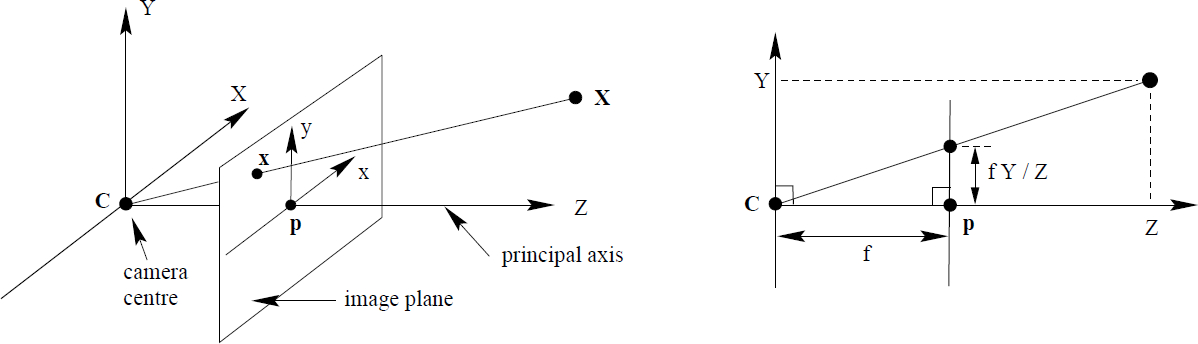
\includegraphics[width=\textwidth]{figures/pinhole_camera.jpg} 
	\caption{Perspektívna projekcia štrbinovou kamerou.}
	\label{fig:pinhole_camera}
\end{figure}

Na obrázku \ref{fig:pinhole_camera} je znázornená geometria dierkovej kamery. Stredom projekcie je optické centrum. Kolmica medzi optickým centrom a obrazovou rovinu $\pi$ sa nazýva hlavná os $Z$. Hlavným bodom $p$ je miesto, v ktorom os $Z$ pretína obrazovú rovinu. Rovina prechádzajúca stredom kamery rovnobežne s rovinou obrazu sa nazýva hlavná rovina kamery. $C$ reprezentuje stred kamery (stred perspektívneho premietania). Za predpokladu, že svetové a obrazové body sú zastúpené v homogénnych súradniciach, potom sa stredná projekcia môže jednoducho vyjadriť ako lineárne mapovanie medzi ich homogénnymi súradnicami.

\begin{figure}[h]
	\centering
	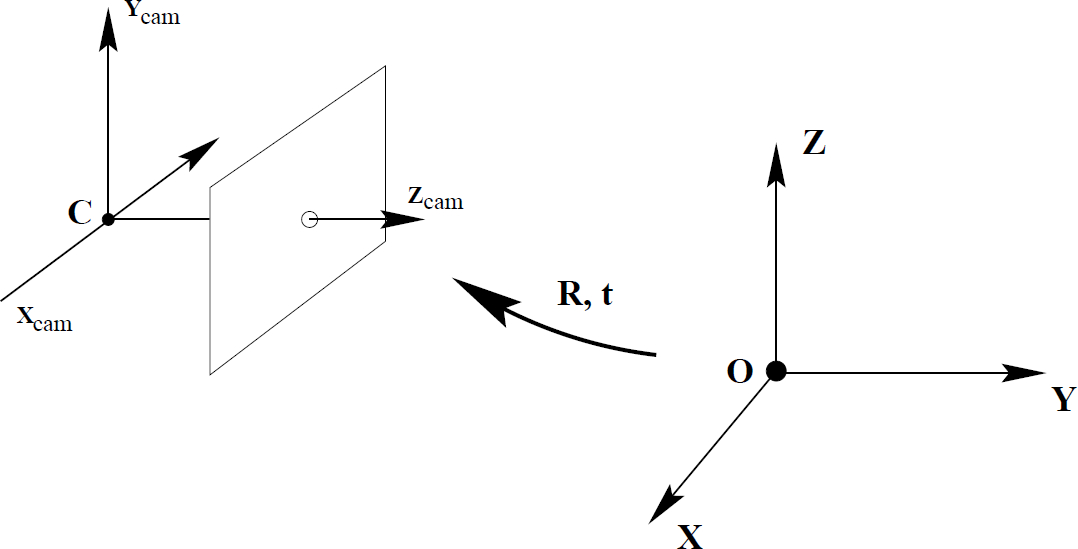
\includegraphics[width=0.7\textwidth]{figures/rotat_translat.jpg} 
	\caption{Vzťah medzi svetovou súradnicovou sústavou a súradnicovou sústavou kamery.}
	\label{fig:rotat_translat}
\end{figure}

Prevod medzi svetovou súradnicovou sústavou (SSS) a kamerovou súradnicovou sústavou (KSS) je zobrazený na obr. \ref{fig:rotat_translat} predstavený vzťahom \ref{eq::pinhole::world_camera}.\newline 

\begin{equation}
\label{eq::pinhole::world_camera}
\begin{aligned}
\begin{bmatrix}
X_{cam} \\ Y_{cam} \\ Z_{cam} \\ 1
\end{bmatrix}=
\boldsymbol{RT}
\begin{bmatrix}
X \\ Y \\ Z \\ 1
\end{bmatrix}
\end{aligned}
\end{equation}

\newpage
\textbf{Svetová súradnicová sústava} je reprezentovaná trojrozmerným karteziánskym súradnicovým systémom, kde stred sústavy $O$ (prípadne $O_w$) je v bode [0,0,0]. Vektory $X,Y,Z$ prislúchajúce k jednotlivým súradniciam sú na seba kolmé. Definujú polohu objektu v scéne. Udávajú sa v dĺžkových jednotkách $[m]$ alebo $[mm]$.\newline 

\textbf{Súradnicová sústava kamery} je reprezentovaná trojrozmerným súradnicovým systémom v bode $C$ (poprípade $O_c$), čo predstavuje stred kamery. Optická os $Z_c$ je daná vektorom pohľadu kamery. Vzťah medzi svetovou súradnicovou sústavou a súradnicovou sústavou kamery je popísaný transláciou $t$ a rotáciou $R$. Vektory sú označené ako $(X_{cam},Y_{cam},Z_{cam})$ \newline 

Body zo súradnicovej sústavy kamery je následne potrebné premietnuť do roviny obrazu $\pi$. Nech je stred premietania pôvodom euklidovského súradnicového systému a obrazová (ohnisková) rovina $Z=f$. Podľa modelu dierkovej kamery na obr. \ref{fig:pinhole_camera} sa bod v priestore so súradnicami $\left(X,Y,Z\right)^T$ mapuje na bod v rovine obrazu $\left(f\frac{X}{Z}, f\frac{Y}{Z}, f \right)^T$ pomocou podobnosti trojuholníkov. Ignorovaním výsledných súradníc obrazu dostávame vzťah ktorý popisuje mapovanie centrálnej projekcie zo svetovej súradnicovej sústavy do obrazovej súradnicovej sústavy.

\begin{equation}
\label{eq::pinhole::camera_iplane::a}
\begin{aligned}
\frac{X_{cam}}{x}=\frac{Z_{cam}}{f}; \frac{Y_{cam}}{y}=\frac{Z_{cam}}{f}
\end{aligned}
\end{equation}

\begin{equation}
\label{eq::pinhole::camera_iplane::b}
\begin{aligned}
x=f\frac{X_{cam}}{Z_{cam}}; y=f\frac{Y_{cam}}{Z_{cam}}
\end{aligned}
\end{equation}

Rovnice \ref{eq::pinhole::camera_iplane::a} a \ref{eq::pinhole::camera_iplane::a} môžeme prepísať do maticového tvaru

\begin{equation}
\label{eq::pinhole::camera_iplane}
\begin{aligned}
\begin{bmatrix}
fX_{cam} \\ fY_{cam} \\ Z_{cam}
\end{bmatrix}
= Z_{cam}
\begin{bmatrix}
x \\ y \\ 1
\end{bmatrix}
=
\begin{bmatrix}
f & 0 & 0 & 0 \\
0 & f & 0 & 0 \\
0 & 0 & 1 & 0 \\
\end{bmatrix}
\begin{bmatrix}
X_{cam} \\ Y_{cam} \\ Z_{cam} \\ 1 
\end{bmatrix}
\end{aligned}
\end{equation}

\textbf{Rovina obrazu} aj \textbf{súradnicový systém obrazových bodov} predstavuje dvojrozmerný priestor. Rozdielom je, že prvý spomenutý systém má počiatok v hlavnom bode a jednotka súradnicového systému je v milimetroch. Druhý spomenutý je reprezentovaný jednotkou pixel, počiatok súradnicového systému je na pozícii $\left(u,v\right)=\left[0,0\right]$. Preto je potrebné transformovať prvý súradnicový systém do druhého. 

\begin{figure}[h]
	\centering
	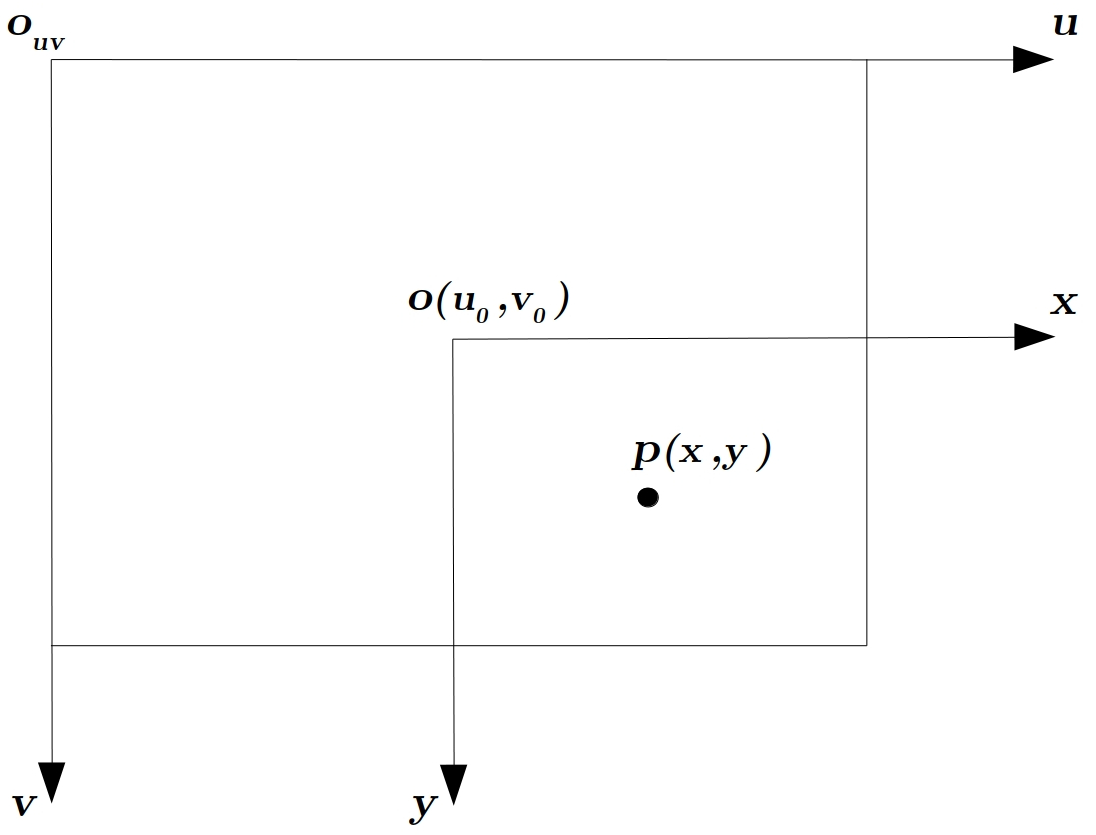
\includegraphics[width=0.45\textwidth]{figures/plane_pixel.jpg} 
	\caption{Vzťah roviny obrazu a súradnicového systému obrazových bodov.}
	\label{fig:plane_pixel}
\end{figure}

Z obr. \ref{fig:plane_pixel} je definovaný hlavný bod $p=o(u_0,v_0)$ (bod, ktorým prechádza hlavná os $Z_{cam}$ v obr. \ref{fig:pinhole_camera}). Pre prevod potrebujeme poznať hustotu pixelov na jednotku dĺžky. Tá je určená pomerom počtu pixelov a rozmerom snímacej plochy v jednotlivých smeroch. Pridaním offsetu $u_0$ a $v_0$ dostávame transformačný vzťah

\begin{equation}
\label{eq::pinhole::plane_pixel}
\begin{aligned}
u=\frac{x}{d_x} + u_0; v=\frac{y}{d_x} + v_0
\end{aligned}
\end{equation}

Z rovnice \ref{eq::pinhole::plane_pixel} získavame kalibračnú maticu $K$, ktorá je zložená z ohniskových vzdialeností $f_x, f_y$ a hlavných bodov $p_x, p_y$. Do úplnej matice $K$ patrí aj koeficient skosenia $s$, ktorý je zvyčajne 0. Táto matica je zložená z takzvaných vnútorných parametrov kamery.

\begin{equation}
\label{eq::pinhole::intrinsic}
\begin{aligned}
K=
\begin{bmatrix}
\frac{x}{d_x} & s & u_0 \\
0 & \frac{y}{d_y} & v_0 \\
0 & 0 & 1 \\
\end{bmatrix}
\begin{bmatrix}
f & 0 & 0 & 0 \\
0 & f & 0 & 0 \\
0 & 0 & 1 & 0 \\
\end{bmatrix}
=
\begin{bmatrix}
f_x & s & p_x & 0 \\
0 & f_y & p_y & 0 \\
0 & 0 & 1 & 0 \\
\end{bmatrix}
\end{aligned}
\end{equation}

Matica kamery $P$ sa skladá z vnútorných a vonkajších parametrov. Matica $R$ zastupuje rotáciu a $t$ transláciu, čo sú vonkajšie parametre (obr. \ref{fig:rotat_translat}). Matica $K$ zastupuje vnútorné parametre.

\begin{equation}
\label{eq::pinhole::p}
\begin{aligned}
\boldsymbol{P}=
\boldsymbol{
K
\begin{bmatrix}
R & t
\end{bmatrix}}=
\begin{bmatrix}
f_x & 0 & p_x \\
0 & f_y & p_y \\
0 & 0 & 1 \\
\end{bmatrix}
\begin{bmatrix}
r_{11} & r_{12} & r_{13} & t_{1} \\
r_{21} & r_{22} & r_{23} & t_{2} \\
r_{31} & r_{32} & r_{33} & t_{3} \\
\end{bmatrix}
\end{aligned}
\end{equation}

Celý prevod je teda možné vyjadriť podľa rovnice \ref{eq::pinhole::full} 
\begin{equation}
\label{eq::pinhole::full}
\begin{aligned}
Z_{cam}
\begin{bmatrix}
u \\ v \\ 1
\end{bmatrix}
=
\begin{bmatrix}
f_x & 0 & p_x \\
0 & f_y & p_y \\
0 & 0 & 1 \\
\end{bmatrix}
\begin{bmatrix}
r_{11} & r_{12} & r_{13} & t_{1} \\
r_{21} & r_{22} & r_{23} & t_{2} \\
r_{31} & r_{32} & r_{33} & t_{3} \\
\end{bmatrix}
\begin{bmatrix}
X \\ Y \\ Z \\ 1
\end{bmatrix}
\end{aligned}
\end{equation}

ktorá je základným matematickým opisom dierkovej kamery a prevodu svetový súradníc do súradnicového systému obrazových bodov. 

\section{Skreslenie šošoviek}

V reálnych kamerách sa vyskytuje určité typy nelineárneho skreslenia, ktoré sú spôsobené pridaním šošovky do ideálnej kamery. Tieto skreslenia spôsobujú nesprávnu perspektívnu projekciu, čím sa následne stráca presná informácia o snímanej scéne. Tieto skreslenia je však možné odstrániť získaním vnútorných parametrov kamery. Medzi najčastejšie skreslenia patria radiálne a tangenciálne skreslenie. 

\subsection{Radiálne skreslenie}
Je spôsobené, keď svetelné lúče ohnú viac v blízkosti okrajov šošovky ako v optickom centre. Čím je objektív menší, tým väčšie je skreslenie. Typickými radiálnymi skresleniami sú súdkovité a poduškové. Koeficienty radiálneho skreslenia modelujú tento typ skreslenia. Deformované body sú označené ako $x'$ a $y'$. Prvky $k_1$ až $k_6$ predstavujú koeficienty radiálneho skreslenia. 

\begin{figure}[h]
	\centering
%	\url{http://www.lightcrafttech.com/support/doc/lens-grapher/how-to-use/}
	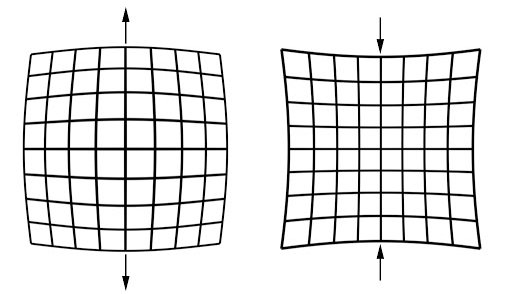
\includegraphics[width=0.68\textwidth]{figures/radial_distortion.jpg} 
	\caption{Radiálne skreslenie spôsobené zakrivením šošovky}
	\label{fig:radial_distortion}
\end{figure}

Neskreslené pixely označené $x$, $y$ sa nachádzajú v normalizovaných súradniciach obrázka. Normalizované súradnice sú vypočítané zo súradníc pixelov preložením do optického stredu a prepočítané pomocou ohniskovej vzdialenosti v pixeloch. Takže $x$ a $y$ sú bezrozmerné.

\begin{equation}
\label{eq::radial_dist::a}
\begin{aligned}
x'= x \frac{1 + k_{1}r^{2} + k_{2}r^{4} + k_{3}r^{6}}{1 + k_{4}r^{2} + k_{5}r^{4} + k_{6}r^{6}}
\end{aligned}
\end{equation}

\begin{equation}
\label{eq::radial_dist::b}
\begin{aligned}
y'= y \frac{1 + k_{1}r^{2} + k_{2}r^{4} + k_{3}r^{6}}{1 + k_{4}r^{2} + k_{5}r^{4} + k_{6}r^{6}}
\end{aligned}
\end{equation}

\begin{equation}
\label{eq::radial_dist::c}
\begin{aligned}
r^2=x^2+y^2
\end{aligned}
\end{equation}

Ak je $k_1<0$ , tak je skreslenie súdkovité a ak $k_1> 0$, tak ide o skreslenie poduškovité. Koeficienty $k_3$ a vyššie sú pri bežných deformáciách zvyčajne rovné 0. Prejavujú sa prevažne pri širokouhlých objektívoch. $r$ reprezentuje rádius k hlavnému bodu, kde nie je skreslenie.  

\subsection{Tangenciálne skreslenie}

Tangenciálne skreslenie vzniká pri neparalelnom umiestnení senzora kamery so šošovkou. Koeficienty $p_1$ a $p_2$ predstavujú tangenciálne skreslenie šošovky:

\begin{figure}[h]
	\centering
	%	\url{https://www.researchgate.net/figure/Tangential-distortion_fig5_332199146}
	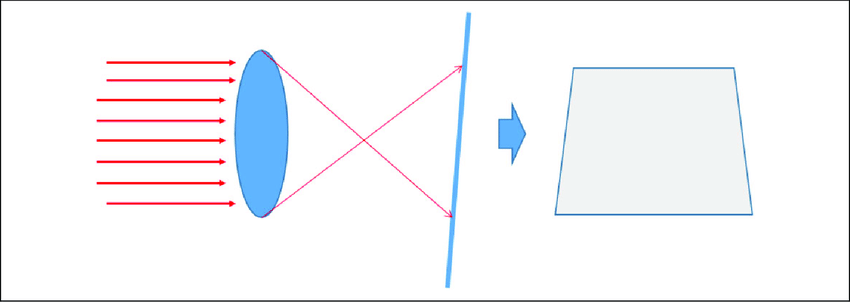
\includegraphics[width=0.7\textwidth]{figures/tangential_distortion.png} 
	\caption{Tangenciálne skreslenie spôsobené nesprávnym umiestnením šošovky}
	\label{fig:tangential_distortion}
\end{figure}

\begin{equation}
\label{eq::tangential_dist::a}
\begin{aligned}
x'= 2p_{1}xy + p_{2}\left(r^{2} + 2x^{2}\right)
\end{aligned}
\end{equation}

\begin{equation}
\label{eq::tangential_dist::b}
\begin{aligned}
y'= p_{1}\left(r^{2} + 2x^{2}\right) + 2p_{2}xy
\end{aligned}
\end{equation}

\begin{equation}
\label{eq::tangential_dist::c}
\begin{aligned}
r^2=x^2+y^2
\end{aligned}
\end{equation}

\subsection{Model reálnej kamery s korekciou skreslenia šošoviek}

V reálnych podmienkach je model ideálnej (dutinkovej) kamery doplnený o rovnice korekcie skreslenia šošoviek, tangenciálneho a radiálneho. Potreba získania koeficientov kamery je veľmi dôležitá z hľadiska správnej spätnej rekonštrukcie 2D obrazu do 3D priestoru.

\begin{equation}
\label{eq::real_camera::a}
\begin{aligned}
\begin{bmatrix}
u \\ v \\ z
\end{bmatrix} = R
\begin{bmatrix}
X \\ Y \\ Z
\end{bmatrix} + t 
\end{aligned}
\end{equation}

\begin{equation}
\label{eq::real_camera::b}
\begin{aligned}
x'= \frac{x}{z}; y'= \frac{y}{z}
\end{aligned}
\end{equation}

\begin{equation}
\label{eq::real_camera::d}
\begin{aligned}
x''= x' \frac{1 + k_{1}r^{2} + k_{2}r^{4} + k_{3}r^{6}}{1 + k_{4}r^{2} + k_{5}r^{4} + k_{6}r^{6}} + 2p_{1}x'y' + p_{2}\left(r^{2} + 2x'^{2}\right)
\end{aligned}
\end{equation}

\begin{equation}
\label{eq::real_camera::e}
\begin{aligned}
y''= y' \frac{1 + k_{1}r^{2} + k_{2}r^{4} + k_{3}r^{6}}{1 + k_{4}r^{2} + k_{5}r^{4} + k_{6}r^{6}} + p_{1}\left(r^{2} + 2y'^{2}\right) + 2p_{2}x'y'
\end{aligned}
\end{equation}


\begin{equation}
\label{eq::tangential_dist::f}
\begin{aligned}
u = f_{x} x'' + c_{x}; v = f_{y} y'' + c_{y}
\end{aligned}
\end{equation}


\section{Kalibrácia}

Kalibrácia kamery je nevyhnutný krok v 3D spracovaní obrazu, kde sa získavajú metrické informácie z 2D obrazov. Kalibráciu môžeme rozdeliť na 3 základné kategórie.

\textbf{Kalibrácia pomocou korešpondencie bodov v 3D priestore}\newline
Kalibrácia kamery sa vykonáva pozorovaním kalibračného objektu, ktorého geometria v 3D priestore je známa s veľmi presnou presnosťou. Kalibráciu je možné vykonať veľmi efektívne. Kalibračný objekt sa obvykle skladá z dvoch alebo troch rovín kolmých na seba.
%O. Faugeras,Three-Dimensional Computer Vision: A Geometric Viewpoint.MITPress, 1993.

\textbf{Autokalibrácia}
Táto technika nepoužíva žiadny kalibračný objekt. Posunutím kamery v statickej scéne je možné vypočítať vnútorné parametre kamier. Ak sú snímky zosnímané tou istou kamerou s pevnými vnútornými parametrami, korešpondencia medzi tromi obrázkami je dostatočná na vypočítanie interných aj externých parametrov, ktoré nám umožňujú rekonštruovať 3D štruktúru. 

\textbf{Kalibrácia pomocou 2D roviny v 3D priestore}




Parametre kamery sa skladajú z vnútorných (intrinsických), vonkajších (extrinsických) koeficientov a koeficientov skreslenia (distortion). K určeniu je potrebné mať 3D body scény (world points) a ich zodpovedajúce 2D body. Získanie týchto korešpondujúcích dát je možné extrakciou ľahko identifikovateľných bodov. Jedným z najpoužívanejších kalibračných vzorov je šachovnica, kde je výrazný farebný prechod medzi hracími poľami (8).



%\section{Planárna homografia}
%Ide o lineárnu perspektívnu transformáciu, ktorá prevádza pixel z jednej roviny $X$ do druhej $X'$ v projektívnom priestore. 
%Homografia je využiteľná 3 spôsobmi:
%
%\begin{description}[leftmargin=*,labelsep=5.8mm, font=$\bullet$~\normalfont\scshape\color{black}]
%	\item Prevod roviny v 3D svetových súradniciach do 2D priestoru obrazovej roviny
%	\item Projektová transformácia, zobrazenie 3D plochy dvoma kamerami
%\end{description}
%
%\begin{equation}
%\label{eq_planar}
%\begin{aligned}
%X'=H \cdot X =
%\begin{bmatrix}
%x' \\ y' \\ 1 
%\end{bmatrix}
%= H
%\begin{bmatrix}
%x \\ y \\ 1 
%\end{bmatrix} =
%\begin{bmatrix}
%h_{11} & h_{12} & h_{13}  \\
%h_{21} & h_{22} & h_{23}  \\
%h_{31} & h_{32} & h_{33}  \\
%\end{bmatrix}
%\begin{bmatrix}
%x \\ y \\ 1 
%\end{bmatrix}
%\end{aligned}
%\end{equation}
%
%$H$ je  matica  rozmeru  3x3  a  má  8  nezávislých  parametrov.  Minimálny  počet štyroch  bodov zodpovedajúcich párov (N=4) je potrebných na zabezpečenie riešenia v rámci dovoleného rozsahu. Na spoľahlivé riešenie je potrebné mať viac ako 4 páry.
%
%
%
%Z kalibrácie je možné získať informácie o:
%
%\begin{description}[leftmargin=*,labelsep=5.8mm, font=$\bullet$~\normalfont\scshape\color{black}]
%	\item relatívnej polohe fotoaparátu a snímaného objektu 
%	\item chybe reprojekcie 3D objektu v 2D rovine 
%	\item chybe estimácie parametrov
%\end{description}
%
%Ku kalibrácií sa používa model štrbinovej kamery (pinhole camera model) a skreslenie šošoviek. Model štrbinovej kamery nezohľadňuje skreslenie šošoviek, pretože ideálna kamera nemá objektív (21)
%
%

